\subsection{Valgrind} \begin{frame}{Valgrind}
	\begin{itemize}
		\item Valgrind ist ein Framework um dynamische Analyseprogramme (Tools) zu entwickeln.
		\pause \item Valgrind ist eine virtuelle Maschine und JIT Compiler.
		\pause \item Valgrind verwendet Dynamic Binary Translation (DBT) 
		\pause \item Tools führen Analyse und/oder Instrumentierung durch.
		\pause \item{\bf Tools:} Memcheck, Cachegrind, Callgrind, {\bf McTracer} 
	\end{itemize}
\end{frame}

\subsection{Valgrind Workflow}

\begin{frame}{Valgrind Workflow}
	\begin{enumerate}
		\item Das Programm wird eingelesen und in die Vex Intermediate Representation (Vex IR) ueberfuehrt.
		\pause \item IRSB's (IR Super Block) werden an das Skin uebergeben. 
		\pause \item Das Skin instrumentiert/analysiert die IRSB's.
		\pause \item Die IRSB's werden zu Maschinencode kompiliert und nativ ausgefuehrt. 
	\end{enumerate}
\end{frame}

\begin{frame}{Darstellung des Maschinencodes in Vex IR}
	\lstset{frame=single}
	\lstinputlisting[language=C, basicstyle=\tiny]{mctracer/irsb.c}
\end{frame}

\begin{frame}{Instrumentierung}
	\lstset{frame=single}
	\lstinputlisting[language=C, basicstyle=\tiny]{mctracer/instrument.c}	
\end{frame}

\subsection{Valgrind Client Requests}

\begin{frame}{Valgrind Client Requests}
	\begin{itemize}
		\item Client Requests erlauben dem analysierten Programm mit Valgrind bzw. dem Tool zu kommunizieren.
		\pause \item Client Requests sind ein Trapdoor Mechanismus.
		\pause \item Werden bei McTracer verwendet um die zu analysierenden Datenstrukturen festzulegen.
	\end{itemize}

	\pause

	\lstset{frame=single}
	\lstinputlisting[language=C, basicstyle=\tiny]{mctracer/client_example.c}
\end{frame}

\begin{frame}{Valgrind Client Requests}
	\lstset{frame=single}
	\lstinputlisting[language=C, basicstyle=\tiny]{mctracer/client_impl.c}	
\end{frame}


\begin{frame}
        \begin{block}{Stille Annahmen und Beschränkungen}
                \begin{itemize}
                        \pause \item Ein Zugriff ist nie Größer als eine Cachezeile
                               \item Ein Zugriff fällt nie in mehr als zwei Cachezeilen
                        \pause \item Alle Elemente einer Matrix sind gleich groß
                        \pause \item Nachbarn in einer Zeile der Matrix liegen im Speicher nebeneinander, übereinanderliegende Zeilen liegen im Speicher nebeneinander
                \end{itemize}
        \end{block}
\end{frame}

\subsection{Eventverarbeitungsstruktur} The GUI is implemented solely in Java, utilizing the Swing Architecture. The project is structured according to the Model–View–Controller pattern. It consists of three packages (\texttt{data}, \texttt{view} and \texttt{controller}), separating the data from the interface, connected through the \texttt{controller}. The package \texttt{data} is responsible for reading the data files and providing a comprehensive interface to retrieve the data. The package \texttt{view} is responsible for displaying the data to the user. It communicates with the data only via the \texttt{controller} (and vice versa). Therefore the \texttt{controller}'s purpose is to manage the entire data flow of the software. It sends requested data to the user interface or requests new data to be loaded from a file. 

\subsection{Class Responsibilities - Package \texttt{view}}
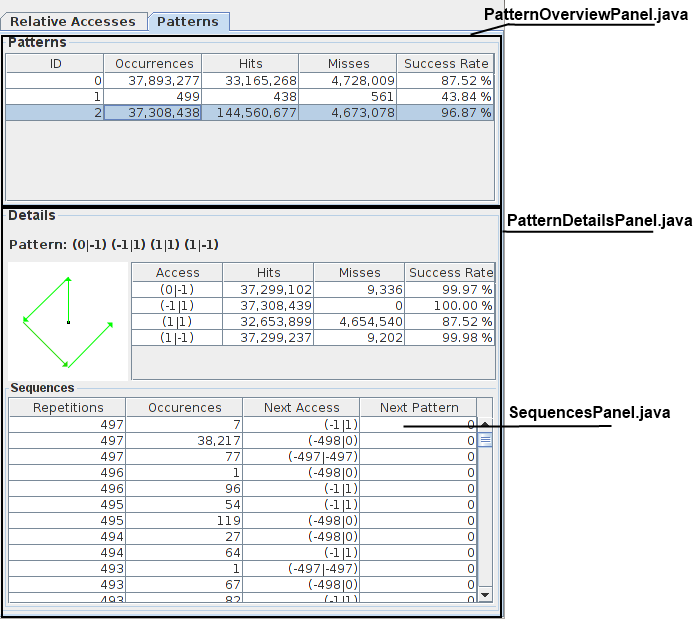
\includegraphics[width=350px]{gui/classresp2.png}
\newpage 
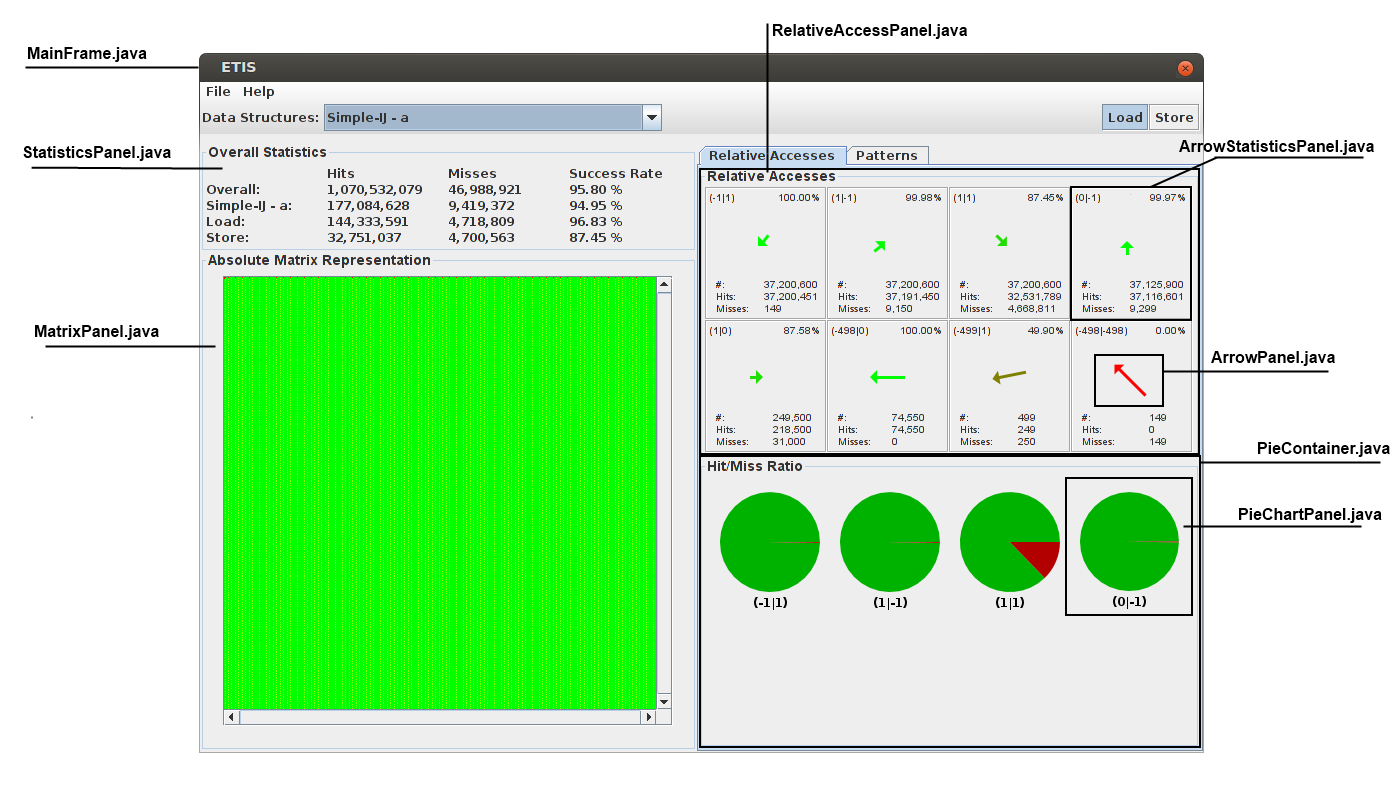
\includegraphics[angle=90,height=700px]{gui/classresp1.png}
\subsection{Informal Class Diagramm}
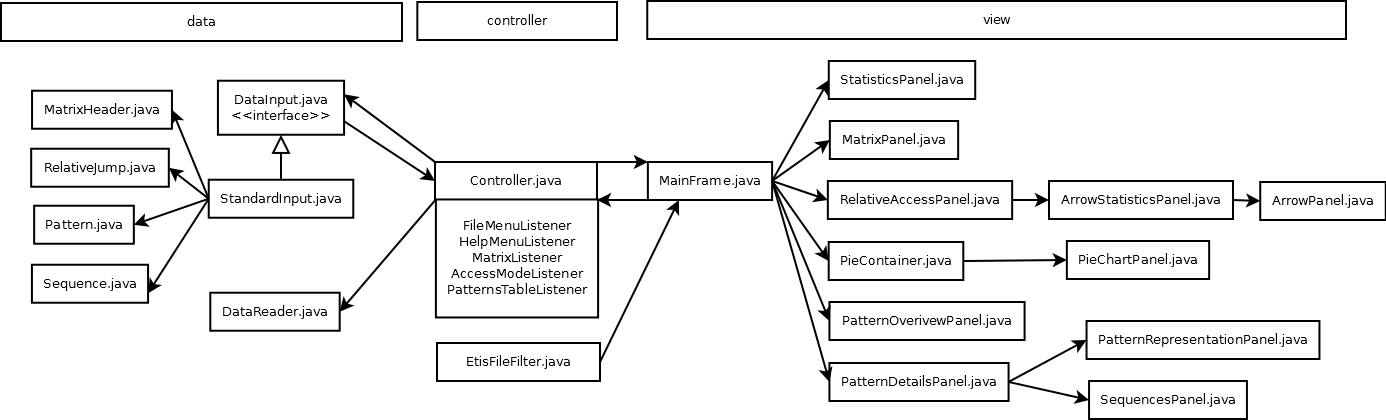
\includegraphics[angle=90,height=560px]{gui/comm.png} 
